\paragraph{} Esta es la página para añadir nuevos elementos en la base de datos de una manera sencilla. En ella aparecen se le presenta al administrador un formulario con los diferentes campos a rellenar de los microcontroladores que son, uno por característica: \textbf{Referencia}, \textbf{Arquitectura}, \textbf{Frecuencia(MHz)}, \textbf{Memoria Flash(KB)}, \textbf{Memoria RAM(KB)} y \textbf{precio (\euro)}.

\paragraph{} Al rellenar todos los campos y pulsar sobre el botón situado a la derecha se añade el elemento a la base de datos y automáticamente se redirigirá al administrador a la página de listado completo, con el nuevo microcontrolador ya incluido en la lista.

\begin{figure}[h!]
	\centering
	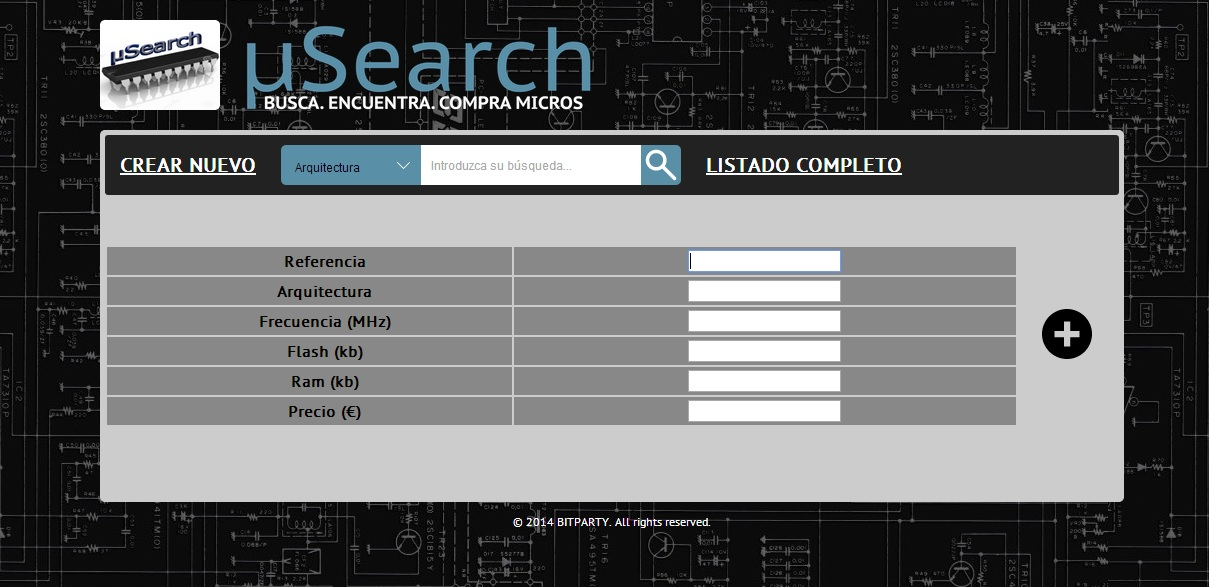
\includegraphics[width=0.75\textwidth]{img/anyadir}
	\caption{Página para añadir un nuevo micro-controlador.}
	\label{fig:anyadir}
\end{figure}

\paragraph{}Además, desde esta página, a través de los iconos situados en la cabecera debajo de los logotipos de la web, el administrador puede acceder a:

\begin{itemize}
	
	\item \textbf{Crear Nuevo:} Recarga la página actual de creación de un nuevo microcontrolador. El formulario actual no se guarda al recargar la página.

	\item \textbf{Búsqueda:} Desde esta sección, el administrador puede realizar búsquedas sobre el catálogo de microcontroladores en base a cualquiera de sus características (Arquitectura, Frecuencia, Flash, RAM). Se debe seleccionar una de las características de la lista despegable, introducir el texto a buscar y pulsar sobre el icono de búsqueda.
	El usuario será redirigido a una página donde se le mostrará el resultado de la búsqueda.
			
	\item \textbf{Listado Completo:} Redirige al administrador a la página en la que se listan todos los microcontroladores disponibles en el catálogo.
\end{itemize}